\begin{center}
  \begin{tabular}{rp{6cm}lp{12cm}}%{rl}
  % after \\: \hline or \cline{col1-col2} \cline{col3-col4} ...
  论文地址:& \href{https://arxiv.org/abs/1808.05689v4}{https://arxiv.org/abs/1808.05689v4} \\
  源码:& \href{https://github.com/yunshengb/SimGNN}{SimGNN} \\
%  slides:& \href{http://yunshengb.com/wp-content/uploads/2017/03/nips_2018_r2l_workshop_talk.pdf}{{\footnotesize Convolutional Set Matching for Graph Similarity}}\\
  关键词:& \textbf{Graph Similarity, GCN, Graph Edit Distance} \\
  写于:& \date{2020-10-13}
  \end{tabular}
\end{center}

该论文\cite{bai2019simgnn}与\ref{sec:GSimCNN}的作者相同,也是为了解决图相似性计算的问题,该论文的方法/模型与\ref{sec:GSimCNN}中的方法/模型类似。论文中提出了SimGNN(Graph  Similarity Computation via Graph Neural Network)来解决这个问题。

\textbf{SimGNN思路}\hspace{12pt}该方法针对图相似性的计算提出了两个策略(strategy),能够分别计算$\mathcal{G}_1, \mathcal{G}_2$的相似性,论文中将这俩策略结合起来一起使用。Strategy 1是通过GCN得到graph-level的图表征,基于图表征计算相似度。Strategy 2是利用图中的结点表征进行相似度的计算。Strategy 1/2 的过程可参考Fig.\ref{fig:SimGNN},细节如下。

\begin{figure}[h]
	\centering
	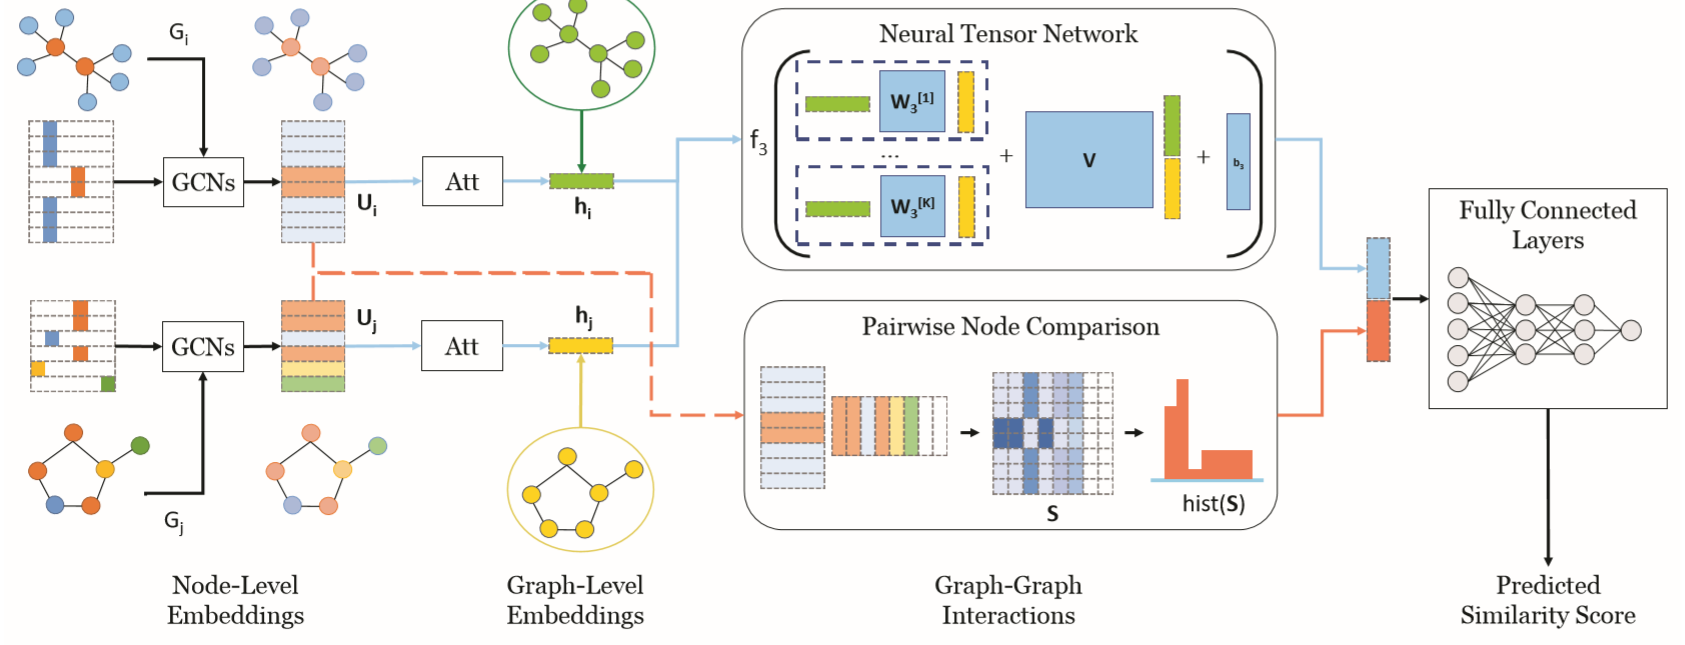
\includegraphics[width=0.8\textwidth]{pics/SimGNN.PNG}
	\caption{SimGNN}
	\label{fig:SimGNN}
\end{figure}

\paragraph{Strategy 1}Strategy 1是通过GCN计算每个结点的表征,再通过注意力的方法计算得到图的表征,该过程又可以分为4个阶段。

\subparagraph{Stage 1}计算节点表征。如Fig.\ref{fig:SimGNN}所示,通过GCN(论文中使用的\href{https://github.com/mdeff/cnn_graph}{GCN})计算得到每个结点的表征。

\subparagraph{Stage 2}计算图表征。SimGNN是以结点表征为基础,基于注意力计算图表征的。在计算图表征之前,先计算图的上下文(global  graph context)--- 上下文向量$\boldsymbol{c} = tanh(\frac{1}{N} \boldsymbol{W_2} \sum_{n=}^N \boldsymbol{u_n})$,其中$\boldsymbol{W_2}$是待学习得参数。对于任意一个结点$\boldsymbol{u_n}$,它的注意力(权重)计算方式是:$attention(\boldsymbol{u_n}) = \sigma( \boldsymbol{u_n}^\mathrm{T} \boldsymbol{c} )$。最终图$\mathcal{G}$的表征$\boldsymbol{h} = \sum_{n=1}^{N} attention(\boldsymbol{u_n}) \boldsymbol{u_n}$。

论文中特别提到了一个点 --- 没有对$attention(\boldsymbol{u_n})$进行归一化,即虽然$attention(\boldsymbol{u_n}), \forall n \in \{1, ... , N\}$是在0到1之间的,但是没有经过一个类似softmax的归一化。这是为什么呢?难道总的权重不应该为1吗?论文中给出的解释是:让最后得到的图表征反映图的大小,这对相似性计算是很重要的。很巧妙,{\color{red}并不是所有的情况都需要归一化}!
 
\subparagraph{Stage 3}使用图表征计算 Graph-Graph interaction。这里的图交互(个人翻译),指的是通过图表征计算一个相似度向量。具体操作:使用Neural Tensor Network(NTN)来对图表征之间的关系进行建模。则两个图表征之间的关系表示为$g(\boldsymbol{h_i}, \boldsymbol{h_j}) = f( \boldsymbol{h_i}^\mathrm{T} \boldsymbol{W_3^{[1:K] } } \boldsymbol{h_j} + \boldsymbol{V} \begin{bmatrix}
	\boldsymbol{h_i} \\ \boldsymbol{h_j}
\end{bmatrix} + \boldsymbol{b_3} )$。其中$\boldsymbol{W_3^{[1:K] } }$是一个张量,包括$\boldsymbol{V}和\boldsymbol{b_3}$都是待学习的参数,K是超参数,最后$g(\boldsymbol{h_i}, \boldsymbol{h_j})$的结果就是一个$\mathbb{R}^K$中的相似度向量。

\subparagraph{Stage 4}计算图相似度。从stage 3 得到两幅图的相似度向量后使用全连接的MLP计算相似度。
\newline

以上4个阶段就是Strategy 1 的全过程,使用图标表征的interacting能够反映相似度基于这样一个假设:好的图表征应该能够编码图的结构和特征信息,可以通过图表征的interacting来预测图之间的相似性({\color{red}为什么通过interacting就能反映图之间的相似性呢?})。

\paragraph{Strategy 2}使用GCN输出的结点表征,计算一个与\ref{sec:GSimCNN}中类似的相似矩阵,可以得到一个更细粒度(fine-grained)的相似评估。因为图的结点没有一个特定的排列,Strategy 2使用了一种结点排列无关的方法 --- 提取相似矩阵的直方图特征,来利用相似矩阵计算相似度。直方图的bin的数量是超参数。

将Strategy 1 和 Strategy 2结合起来使用时将Strategy 1中stage 3得到的相似度向量与Strategy 2得到的直方图特征(也是一个向量)拼接后输入到全连接的MLP中计算得到一个相似度。
\newline

至此,SimGNN的过程就说完了。总的来说,Strategy 1是从粗粒度上来计算图之间的相似性,而Strategy 2则是从更细粒度上计算结点相似性,Strategy 2能够对Strategy 1进行补充、增强(但论文中的实验说明,使用Strategy 2后并没有较大的提升)。

\paragraph{方法解决的问题/优势}
\begin{itemize}
	\item SimGNN计算相似性是结点排列无关的。也就是说,同一个图,不同的结点排列,不会影响它和其他图的相似性的计算。这主要是因为使用了相似矩阵的直方图特征
	\item 模型是inductive的,能够泛化到未见过的图。SimGNN中使用的GCN是inductive的
	\item SimGNN是end-to-end的模型,参数都是可学习的
\end{itemize}

\paragraph{方法的局限性/未来方向}
\begin{itemize}
	\item 在Strategy 2中使用直方图特征虽然是结点排列无关的,但个人认为不能充分地利用相似矩阵,这也可能是为什么Strategy 2效果不明显地原因。或许有更好的结点排列无关的方法来利用结点表征(并不一定要使用相似矩阵)
	\item 图上下文向量$\boldsymbol{c}$的原因,为什么使用它?
	\item SimGNN只使用了结点的特征,并没有{\color{red}使用边的特征},后期可以将边的特征纳入模型考虑的范畴。在一些领域,如化学领域,边的类型是很重要的
	\item 目前的图的相似性计算主要针对较小的图,如何计算大规模的图的相似性呢
	\item {\color{red}如何计算更复杂的图的相似性呢,如动态图}
\end{itemize}

作者其他工作可参考\href{http://yunshengb.com/}{他的主页}。

